\chapter{Agent-based workflow for inferring evolutionary parameters from
molecular data using approximate Bayesian computation}\label{chapter:methdemon}


\section{Introduction}
In chapter \ref{chapter:trajectories}, I used a general spatial agent-based
model to investigate broad evolutionary patterns as related to spatial
organisation. While the model was capable of simulating the dynamics of tumour
growth, its utility is limited by the computational cost of simulating a large
number of cells. This means that using the model's outputs in comparison to or
to draw inference from real data is not feasible. \par
There are a few ways to address this issue. For example, rather than simulating
all clones in a tumour, one could take the approach of
\cite{sottoriva_big_2015} and use demes (tumour glands) as the principal agent
of our simulation. This would allow for a realistically-sized tumour to be
generated as the number of glands would be around the right order of magnitude.
A problem with this approach is that it loses resolution since a gland's
population is assumed to be clonal, undergoing rapid fixation in the case of an
emerging mutant. If one wanted to study evolutionary dynamics on a finer scale
it would be necessary to at least simulate the dynamics of cell lineages, if
not individual cells, as performed earlier. \par
In \cite{gabbutt_evolutionary_2023}, the authors employ a stochastic model for
an expanding cell population to model the behaviour of fluctuating CpG sites in
blood cancers. The model is capable of simulating the dynamics and the
corresponding fluctuating methylation arrays of lymphoid malignancies at scale.
However, this model is not spatially explicit, which is a feature that has to
be distinguished between different glands in a solid tumour. In this chapter, I
present a purpose-written agent-based model, \texttt{methdemon}, which reduces
the computational cost of simulating a tumour's growth and models the
fluctuating methylation arrays in colorectal cancer.

\subsection{Fluctuating methylation arrays}
As mathematicians new to biology quickly learn, perfectly clean data containing
detailed information about the population structure of a tumour is
non-existent. In fact, most data is noisy and at best measures a decent proxy
for the properties which can be described by a mathematical model. Therefore,
one learns very quickly to improvise and adapt when working with biological
data. Specifically, when it comes to cancer, a compromise has to be made
between resolution and scale. Where single-cell data can provide a detailed
view of the mutations accumulated in the genome, it is not feasible to obtain
it for a whole tumour. On the other hand, bulk data gives a high-level view of
the tumour's population structure, but a lot of the details get lost in the
process. \par
However, DNA sequencing is not the only way to obtain information about a
tumour's population structure. Early work with methylation arrays in colorectal
cancer has shown potential for inferring the ancestry and age of a tumour
\cite{hong_using_2010, siegmund_high_2011}. In a way the genome shows more
mutations in older populations, methylation arrays will also be more diverse as
time goes on. Current techniques allow for the sequencing of some $850,000$ CpG
sites which, while a small fraction of the genome, is still enough to proide
valuable insight into the underlying dynamics of the cell population. Initial
studies on methylation as a tracker of evolution made use of the whole array
\cite{siegmund_modeling_2008, sottoriva_integrating_2010}. However, more recent
work has shown that just a small subset of CpG sites is enough to infer the
evolutionary dynamics of a cell population \cite{gabbutt_fluctuating_2022,
gabbutt_evolutionary_2023}. This is the set of fluctuating CpG (fCpG) loci,
which is also the topics of chapter \ref{chapter:methylation}. \par
As fCpG loci seem to be a neutral marker of cell population dynamics, I will
define the following set of assumptions for modelling their behaviour:
\begin{enumerate}[(i')]
    \item \textbf{Each cell has a corresponding fCpG array inherited from its
        parent cell.}
    \item \textbf{Upon cell division, each methylated fCpG site has an
        independent and equal probability of being demethylated, and
        vice-versa.}
    \item \textbf{The rates of methylation and demethylation do not change over
        time.}
\end{enumerate}
These assumptions are based on the findings of \cite{gabbutt_fluctuating_2022,
gabbutt_evolutionary_2023}.

\subsection{A comment on using existing models}\label{section:old_famework}

As discussed in section \ref{section:abm}, it is preferable to use established
frameworks and models for simulating tumour growth and evolution. Therefore,
with the assumptions outlined in the previous section, my initial approach was
to employ a general agent-based model with small modifications, to simulate the
behaviour of fCpG loci in cancer. The first model I considered was
\texttt{demon}, with which I had already worked in chapter
\ref{chapter:trajectories}, as its light weight and reasonable wall times had
shown promise. A naive approach to simulating methylation arrays is to use the
model's passenger mutations as a proxy for epigenetic changes. This way, the
model could be run as usual with modified passenger mutation rates, and
methylation arrays could be assigned to the cells post-hoc. The main issue with
this approach is memory management, as the output files tend to be large and
thus difficult to handle in the post-processing steps. This meant that applying
any sort of inference workflow would take a long time, making the approach
impractical. This stands for other SABMs as well, due to the amount of data
produced when simulating a whole tumour's growth.

\section{An ABM of fluctuating methylation arrays in
cancer}\label{section:methdemon}
% \subsection{Overview}
% \begin{itemize}
%     \item go over the simulation's inner workings
%     \item sensitivity analysis
%     \item provide estimates of running efficiency and memory requirements
%     \item discuss possible upgrades and their potential computational costs
% \end{itemize}
To tackle the issue of models generating too much unused data, I wrote a new
ABM, \texttt{methdemon}, capable of simulating a growing cell population and
their corresponding fCpG arrays. The model can be run as a well-mixed population
expansion, or in a 1D spatial setting, with the latter being relevant in the
case of multi-site sequencing of a tumour spheroid. The model is written in C++,
with an emphasis on execution time and dynamic memory management.

\subsection{Model structure}
Inspired by the \texttt{demon} model, event scheduling happens according to the
Gillespie algorithm, with a deme being chosen first, followed by a cell within
that deme. Events are then chosen based on the sum of rates in the tumour,
between cell birth, cell death, and deme fission. Upon cell division, both the
parent and daughter cells have the same probability of acquiring a driver
mutation, and each cell's fCpG array is updated according to the rules outlined
in the previous section. A list of relevant model parameters is given in table
\ref{table:methdemon_params}, with source code and examples available in the
model's github repository \cite{methdemon_repo}.
\begin{table}[h]
    \centering
    \begin{tabularx}{\textwidth}{|c|X|c|}
        \hline
        Parameter & Description & Units \\
        \hline
        \texttt{deme\_carrying\_capacity} & The maximum number of cells in a
        gland & cell \\
        \hline
        \texttt{init\_migration\_rate} & The probability of a gland undergoing
        fission & $\text{cell}^{-1}\text{(cell division)}^{-1}$\\
        \hline
        \texttt{mu\_driver\_birth} & The probability of a cell acquiring a
        driver mutation & $\text{cell}^{-1}\text{(cell division)}^{-1}$ \\
        \hline
        \texttt{s\_driver\_birth} & The selective advantage of a mutant
        cell & n/a \\
        \hline
        \texttt{meth\_rate} & The probability of an unmethylated fCpG site
        changing state & $\text{(cell div)}^{-1}\text{(fCpG site)}^{-1}$\\
        \hline
        \texttt{demeth\_rate} & The probability of a methylated fCpG site
        changing state & $\text{(cell div)}^{-1}\text{(fCpG site)}^{-1}$\\
        \hline
    \end{tabularx}
    \caption{Parameters used in the \texttt{methdemon} model.}
    \label{table:methdemon_params}
\end{table}
 Consider a tumour consisting of $N$ demes at the end of growth. Each deme,
 during growth, has a probability $p$ of undergoing fission, and the final mean
 number of fissions per deme is $\log_2N$. Further, the expected number of
 descendant demes of deme $i$ is given by
\begin{equation}
    \frac{N_i}{N} = \frac{(2pt)^i}{i!}e^{-2pt},
\end{equation}
i.e. the Poisson distribution with mean $2pt$, as derived in
\cite{kharlamov_generation}. This condition governs how fissions are handled in
the model. As a real tumour can consist of millions of glands, the model narrows
the focus to the subset of demes sequenced at the end of growth. Fissions which
produce untracked demes, pseudo-fissions in the model, are the main way of
accumulating fission events in a deme. Each pseudo-fission simply discards half
of the deme's population, stochastically rounded. Real fissions are implemented
by assigning a probability to each fission event of being tracked, equal to
\begin{equation}
    \phi = \frac{p}{\mathbb{E}[\text{fissions per deme}]/2}.
\end{equation}
By using a discrete random distribution, I ensure that the expected number of
fissions before a true fission event in a deme is about half of the mean total
number of fissions. This means, on average, that the deme undergoing the first
true fission is the only deme in the tumour, but also it is unlikely that the
simulation ends with only one deme. Ignoring pseudo-fissions, this is
equivalent to having a fission rate of $p\times\phi$. Pseudo-fissions are
important, however, not just for the purpose of tracking the mean number of
fission events, but also for population dynamics of the demes. Depending on the
deme carrying capacity, that is the maximum number of cells in a deme, and
mutation and epimutation rates, a fission can impact the population structure
of a deme in different ways. Let $K$ be the carrying capacity of a deme, $\mu$
the driver mutation rate, $\gamma$ the epimutation rate, and $L$ the number of
fCpG sites per cell (assuming equal methylation and demethylation rates for
simplicity). Upon fission, the population of the deme is divided into two, and
there need to be $K/2$ cell division events before the deme is back to its
carrying capacity. The expected number of mutations is the simply
$K/2\times\mu$, and the expected number of epimutations is
$K/2\times\gamma\times L$. Depending on the rates, these numbers can be quite
different. Realistically, the number of driver mutations during repopulation of
a deme is likely negligible. While epimutations are more likely, fCpG arrays
are inherited with a high degree of fidelity, and the fCpG distribution in a
deme post-fission is likely to be similar to just before. However, consider now
the neutral case. When a deme is at carrying capacity, its dynamics are
equivalent to a Moran process, meaning the probability of neutral fixation for
a mutant population of $m$ in a deme of carrying capacity $K$ is equalt to
$m/K$, ignoring fissions. However, as cells grow into empty space post-fission
until carrying capcity is reached, fissions increase the probability of neutral
fixation at smaller deme sizes.

\subsection{Stopping conditions}
When simulating the whole tumour, imposing a stopping condition based on the
total cell population is one of the most straightforward ways to end the
simulation. However, as this model is focussed on a subset of relevant cells, I
decided on a few different options for stopping conditions. If the model is run
in the non-spatial setting, the simulation can be terminated after a maximum
number of cells is reached. In the spatial setting, more concretely in the case
of deme fission, the main indicator of a tumour's growth is the mean number of
fissions per deme. This condition is based on the assumption that a tumour's
progression by fission is equivalent to a birth-only branching process, similar
to the model of \cite{sottoriva_big_2015}. The model also has the option of
simulating steady-state turnover of cells in the simulated demes after the
initial growth phase. This is an approximation of a saturation growth regime,
as real tumours are not expected to grow indefinitely.

\subsection{Sensitivity analysis}
% \begin{itemize}
%     \item list and explain the parameters used in the model (can ignore the ones not yet used)
%     \item briefly explain the snakemake workflow used to run the model a bunch of times
%     \item discuss the results of the sensitivity analysis for the parameters:
%     \begin{itemize}
%         \item carrying capacity - lower carrying capacity means higher probability of neutral
%             fixation
%         \item fission rate - higher fission rate means earlier divergence of glands and more
%             time spent in independent turnover so very different arrays at the end of the
%             simulation; conversely, lower fission rates lead to a more recent split and thus
%             more closely related arrays
%         \item mutation rate - higher mutation rates lead to more emerging mutants and possibly
%             more diverse arrays but too high of a mutation rate leads to clonal interference
%             and may even be similar to the neutral case in terms of array diversity
%         \item selective advantage - neutral to weak selection means more diverse arrays in the
%             small deme limit, but strong selection means quick fixation of the mutant and less
%             diversity on the array level
%         \item epimutation rates - too slow switching means less diversity, too fast means
%             complete decoherence and regeression to a normal distribution around $0.5$
%     \end{itemize}
% \end{itemize}
To check whether the model's behaviour is consistent with the expectations, I
wrote a \texttt{snakemake} workflow to test many combinations of the parameters
from table \ref{table:methdemon_params}. The code is available at the github
repository for the workflow, \texttt{walter} \cite{walter}. A summary of the
results is shown in figures \ref{fig:sensitivity_analysis_1} and
\ref{fig:sensitivity_analysis_2}.

\subsubsection{Carrying capacity}
By carrying capacity, I mean the maximum number of cells with proliferative
potential in a gland. This is effectively equivalent to the maximum number of
stem cells, or lineages, which mainain the gland's population. I considered
three different carrying capacities: $10$, $100$, and $1000$. A real tumour
gland contains about $10^5$ cells, but I assume that not all of them are able
to divide indefinitely, rather following a similar structure to real colonic
crypts \cite{cernat_colorectal_2014}. The results follow intuition: higher
carrying capacity leads to less likelihood of neutral fixation but also more
diversity in the presence of selection.

\subsubsection{Fission rate}
The fission rate in this model is tracked per cell, with a gland's fission rate
being the sum of the fission rates of all cells in the gland. In testing, I
considered per cell fission rates of $10^{-5}$, $10^{-4}$, and $10^{-3}$. As a
consequence, the per deme fission rates ranged from $10^{-4}$ to $1$. This led
to a complication in the form of unfinished simulations, as with too low of a
fission rate, the first deme never splits and the simulation never ends. This
is important to note when choosing priors in the ABC workflow. As we only
consider tumours which have grown in a reasonable time, the prior distribution
of fission rates will be chosen with the carrying capacity taken into account.
The results, as expected, show that tumours with a higher fission rate grow
faster than those with a lower fission rate. Further, fCpG array diversity
depends on the fission rate, epigenetic switching rates and the carrying
capacity, as a high fission rate for smaller demes can still produce a diverse
array with a high epimutation rate, where slower fissions still lead to a
diverse array with a relatively low epimutation rate.

\subsubsection{Driver mutation rate and selective advantage}
The driver mutation rate is the probability of a cell acquiring a driver
mutation upon division. The selective advantage is the proliferative advantage
of cells carrying a driver mutation. In testing, I considered driver mutation
rates of $10^{-5}$, $10^{-4}$, and $10^{-3}$, and selective advantages of $0$,
$0.1$, and $1$. For larger deme sizes, the presence of selection seems to lead
to more desynchronised arrays than the neutral case, as neutral fixation is
less likely. However, at very strong selection, array diversity again decreases
as the mutant quickly fixes in the population. Higher mutation rates lead to
more diverse arrays, but too high of a mutation rate leads to clonal
interference and may even be similar to the neutral case in terms of array
diversity.

\subsubsection{Epimutation rates}
The epimutation rates are the probabilities of a fCpG site changing state upon
cell division. In testing, I considered epimutation rates of $10^{-5}$,
$10^{-4}$, and $10^{-3}$. The results are consistent with the findings of
\cite{gabbutt_fluctuating_2022}, where too slow switching means less diversity,
too fast means complete desynchronisation and regression to a normal
distribution around $0.5$.

\begin{figure}[h]
    \centering
    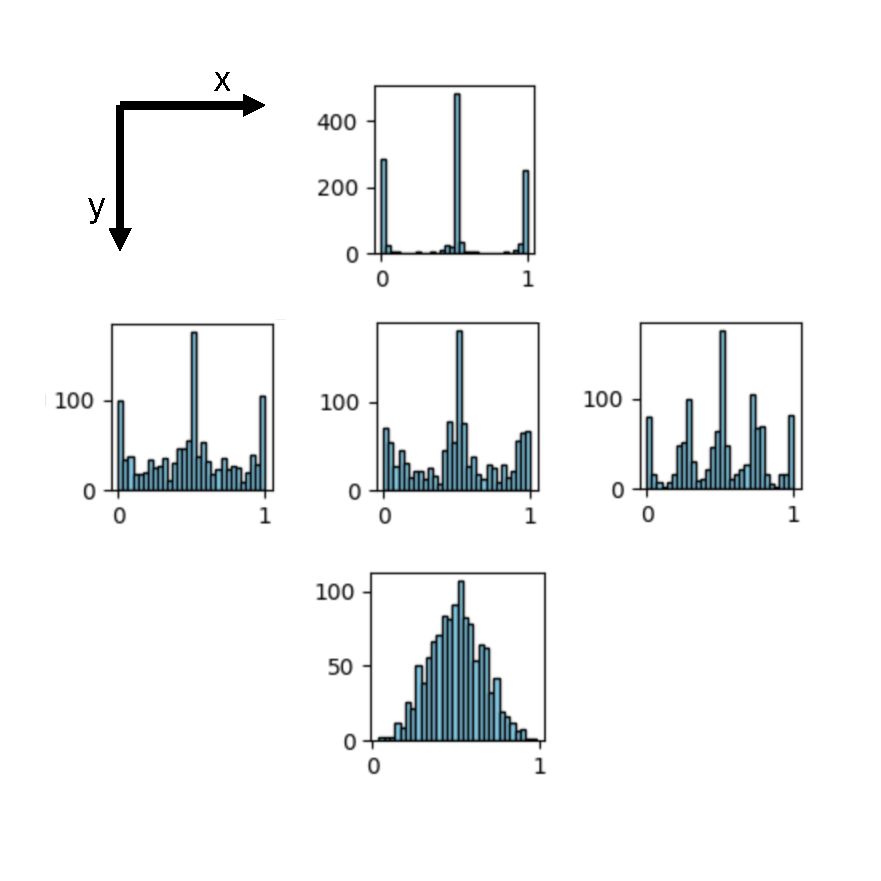
\includegraphics[width=\textwidth]{Chapter_4/figures/sens_fig_1.pdf}
    \caption{Epigenetic mutation rates and strength of selection impact the
    fCpG distribution within a gland. \textbf{x-axis}: selective advantage of
    driver mutations from neutral to weak ($s=0.1$) to strong ($s=0.5$).
    Strong selection leads to clonal interference and fewer dominant lineages,
    reflected in the peaks between $0$ and $0.5$, and $0.5$ and $1$. Neutral
    and weak selection have similar signatures in the simulations, with small
    intermediate peaks emerging occasionally due to the stochastic nature of the
    model and the probability of neutral fixation. \textbf{y-axis}: epimutation
    rates from slowest ($10^{-4}$) to medium ($10^{-3}$) to fastest ($10^{-2}$).
    Slower switching shows very little deviation from the progenitor cell's
    fCpG array, while too fast switching makes the fCpG distribution tend to a
    Gaussian around $0.5$.}
    \label{fig:sensitivity_analysis_1}
\end{figure}

\begin{figure}[h]
    \centering
    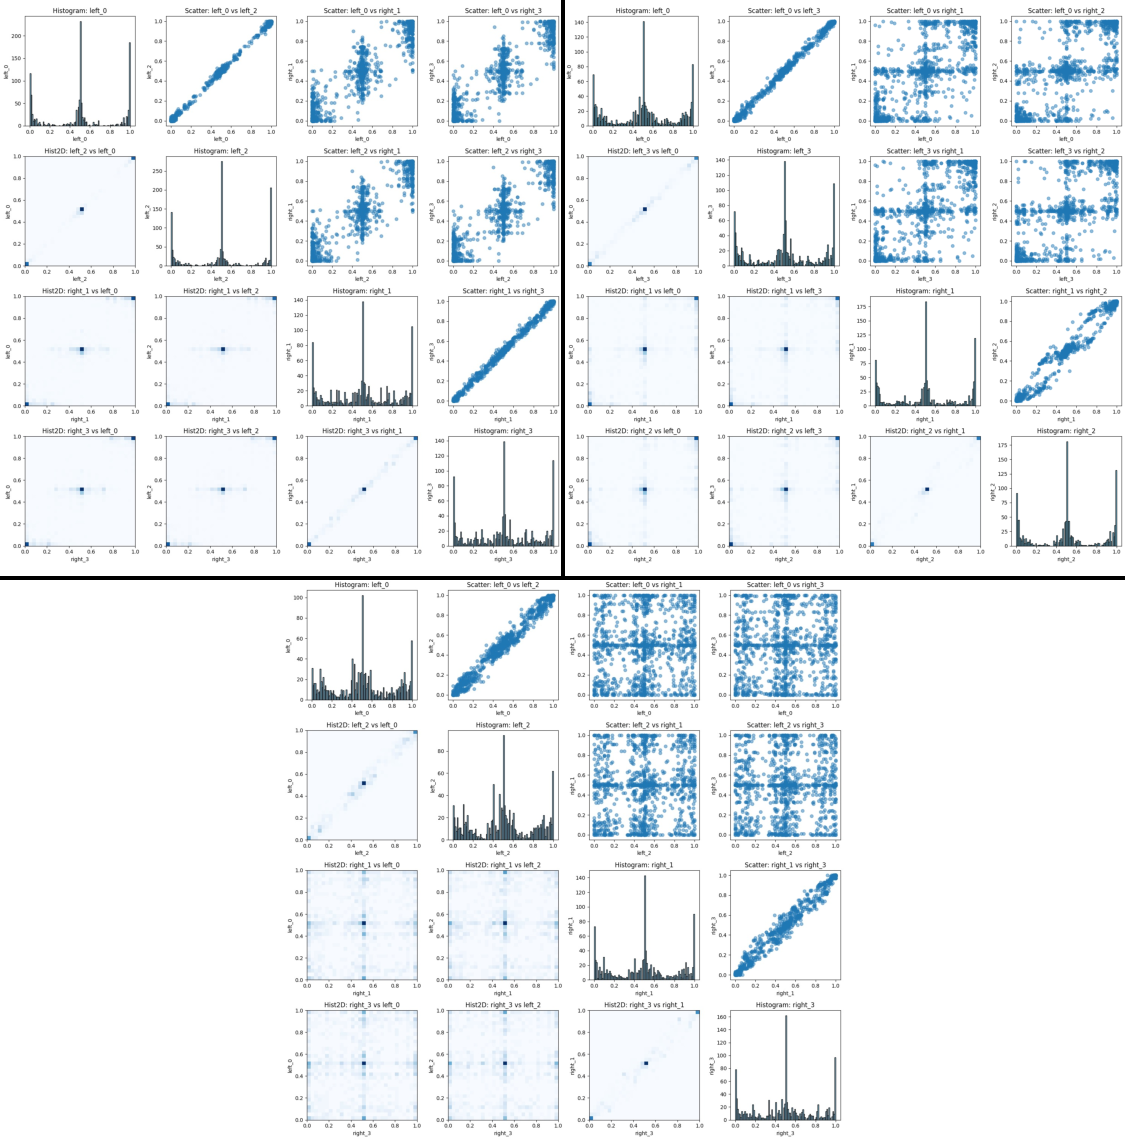
\includegraphics[width=0.8\textwidth]{Chapter_4/figures/sens_fig_2.pdf}
    \caption{}
    \label{fig:sensitivity_analysis_2}
\end{figure}

\subsection{Efficiency and memory requirements}
Apart from standard C++ libraries, the model makes use of the \texttt{boost}
library for random number generation and reading in parameters from a config
file.
\subsubsection{Time complexity}
The model's time complexity is dominated by the fCpG array updates, both in
individual calls and demes. Each fCpG site has an independent probability of
flipping upon division. This means that, if a cell has $L$ fCpG loci, each time
a cell division occurs $2L$ random numbers have to be generated. Consider a
tumour consisting of $N$ demes, each with a carrying capacity of $K$, and with a
target of $F$ mean fissions per deme. If the fission rate per cell is $\phi$, the
expected number of cell births before fission is $1/\phi$.
The time complexity of the model is then
\begin{equation}
    O(F\times N\times K\times L\times\phi^{-1}).
\end{equation}

\subsubsection{Memory usage}
The bulk of the program's memory usage comes from the tracking of each cell's
and deme's fCpG array, with other memory usage being negligible in comparison.
A cell's fCpG array is a $1\times 2L$ vector of integers, where $L$ is the
number of fCpG loci per cell. A deme's fCpG array is a $1\times L$ vector of
floats, calculated as the average of the fCpG arrays of all cells in the deme.
For a tumour of $N$ demes, each with a carrying capacity of $K$, the total
memory used by the program is approximately
$2NKL\times4\text{bytes}+NL\times4\text{bytes}$, for a total memory complexity
of
\begin{equation}
    \theta(NKL).
\end{equation}

\subsubsection{Output files}
The model writes to at least one csv file, and at most two. The compulsory file
contains essential information about the simulated demes and is written at the
end of the simulation or every $10$ generations. This file consists of the
columns:
\begin{itemize}
    \item \texttt{Generation} - time of writing the row
    \item \texttt{Deme} - unique identifier of the deme
    \item \texttt{Parent} - unique identifier of the parent deme
    \item \texttt{Population} - number of cells in the deme at time of writing
    \item \texttt{OriginTime} - time of the deme's birth
    \item \texttt{AverageArray} - the average fCpG array of the deme at time of
        writing
\end{itemize}
The other file contains information about all cells in the simulation and is
written every $10$ generations. This file can be quite large, depending on deme
size, and is not necessary for the inference workflow described in the next
section.

\section{ABC workflow for inferring \texttt{methdemon} parameters}\label{section:methabc}

\subsection{Overview}
For black-box simulations, likelihood-free inference is the most popular method
of parameter estimation. Of these, ABC is preferred by most judging by its
representation in the literature \cite{tavare_inferring_1997,
sottoriva_integrating_2010, sottoriva_big_2015, wang_calibration_2024,
bondi_approximate_2023}. In its most basic form, ABC is a rejection algorithm
which draws parameter values from a prior distribution, simulates data using a
given model, and compares the simulated data to the observed data. If the
distance between the two is less than a given threshold, the parameter values
are accepted. This is repeated until a sufficient number of accepted parameter
values is obtained. The main issue with this approach is that a completely
random search of the parameter space is not efficient, and the number of
simulations required to obtain a sufficient number of accepted parameter values
blows up as the dimension of the parameter space increases. To address this,
the \texttt{pyabc} package was developed \cite{klinger_pyabc_2018,
schalte_pyabc_2022}. The package uses a sequential Monte Carlo algorithm to
sample the parameter space, with the option of using dynamic sampling,
thresholds and particle population sizes for improved efficiency. I decided to
use this package for the inference workflow because of its robust
implementation and intuitive communication with high-performance
infrastructure, such as the City, University of London's cluster, Hyperion.\par
While ABC is a powerful tool for complex models, it is limited by the way data
is compared to simulation outputs. This includes using a summary statistic to
reduce the dimensionality of the data and summarise the most important features
of the output. This also minimises the computational cost of the comparison
step of the workflow. Further, the choice of summary statistic can introduce a
bias, as does the non-zero tolerance threshold. The bias can be reduced with a
smaller threshold, but this increases the overall complexity of the workflow as
more simulations are required to obtain a sufficient number of accepted
parameter values. Additionally, it is difficult to say whether any bias
observed during the inference is due to the inference method or the model
itself.

\subsection{Distance functions}
In the case of the \texttt{methdemon} model, the relevant output data is a set
of average fCpG arrays, one for each deme, at the end of the simulation. As the
fCpG sites fluctuate independently and stochastically, comparing the absolute
values of the arrays is not meaningful. Instead, my focus is on the way arrays
will differ from each other. There are two parts to this approach.

\subsubsection{Inter-gland distance matrix}
To reduce the dimensionality of a single tumour's output, I have defined the
inter-gland distance matrix as a pairwise distance matrix of the average fCpG
arrays of the demes.
\begin{definition}
    Let a simulated tumour consist of $N$ demes, with the array of deme $i$
    given by $\mathbf{a}_i$. The inter-gland distance matrix is then defined as
    \begin{equation}
        D_{ij} = \frac{1}{L}\sum_{k=1}^L(\mathbf{a}_{i}^k-\mathbf{a}_{j}^k)^2,
    \end{equation}
    where $L$ is the number of fCpG sites in the array.
\end{definition}
The idea behind this distance matrix is to emphasise larget differences between
sites, and reduce the impact of small differences. This is done to mitigate the
impact of the noise when comparing the arrays. To compare two distance matrices,
I use the Frobenius norm of their difference.
\begin{definition}
    The distance between two inter-gland distance matrices is defined as
    \begin{equation}
        \delta(D_1, D_2) = \lVert D_1 - D_2 \rVert_F/\sqrt(2) =
        \left(\frac{1}{2}\sum_{i=1}^N\sum_{j=1}^N \lVert a_{ij}
        \rVert^2\right)^{\frac{1}{2}},
    \end{equation}
    where $a_{ij}$ is the element of the difference matrix $D_1-D_2$ at the
    $i$-th row and $j$-th column. The factor of $\sqrt(2)$ is included to
    account for the fact that the matrix is symmetric, and therefore each
    pairwise distance is counted twice.
\end{definition}

\subsubsection{Distance of fCpG distributions}
While the inter-gland distance matrix is an overall measure of the differeces
between two tumours, having independent methylation and demethylation rates
means that the fCpG distribution in a deme can be skewed in different ways. To
make sure that the model is capable of capturing the right relationship between
methylation and demethylation rates, I also compare individual demes' fCpG
distributions using the Wasserstein distance (or the Kantorovich-Rubinstein
metric) \cite{kantorovich_mathematical_1960}. In the context of comparing two
probability distributions, the Wasserstein distance is defined as the minimum
cost of turning one distribution into the other.

\subsection{Example inference}
To demonstrate the utility of the \texttt{methdemon} model and the ABC workflow,
I have performed an example inference using synthetic data generated from the
model. The simulated tumour consists of $8$ demes, each with a carrying capacity
of $100$. The ground truth parameter values and the prior and posterior
distribution of the parameters are shown in table \ref{table:example_inference}.
\begin{table}[htbp]
    \centering
    \begin{tabularx}{\textwidth}{|X|c|c|c|}
        \hline
        Parameter & Ground truth & Prior & Posterior \\ \hline
        Demethylation rate & $0.0018$ & $U[0, 0.5]$ & $0.0091 \pm 0.0046$ \\
        \hline
        Methylation rate & $0.0022$ & $U[0, 0.5]$ & $0.010 \pm 0.005$ \\ \hline
        Fission rate per cell & $0.009$ & $U[0.001, 0.1]$ & $0.056\pm 0.02$ \\
        \hline
        Driver mutation rate & $0.0001$ & $U[0, 0.01]$ & $0.0044 \pm 0.0027$ \\
        \hline
        Selective advantage & $0.1$ & $U[0, 0.5]$ & $0.31\pm0.12$ \\ \hline
    \end{tabularx}
    \caption{Broad priors lead to acceptance of multiple parts of parameter
    space, resulting in broad posterior distributions.}
    \label{table:example_inference}
\end{table}
The inference was performed over $3$ generations using $200$ particles per
generation, with a dynamic tolerance threshold calculated using the
\texttt{SilkOptimalEpsilon} method in the \texttt{pyabc} package. The prior
distribution of the parameters was chosen to be uniform and broad.
Visualisation of the synthetic data is included in the appendix (figure
\ref{fig:synthetic_data_app}). The results of the inference are shown in figure
\ref{fig:example_inference}.
\begin{figure}[h]
    \centering
    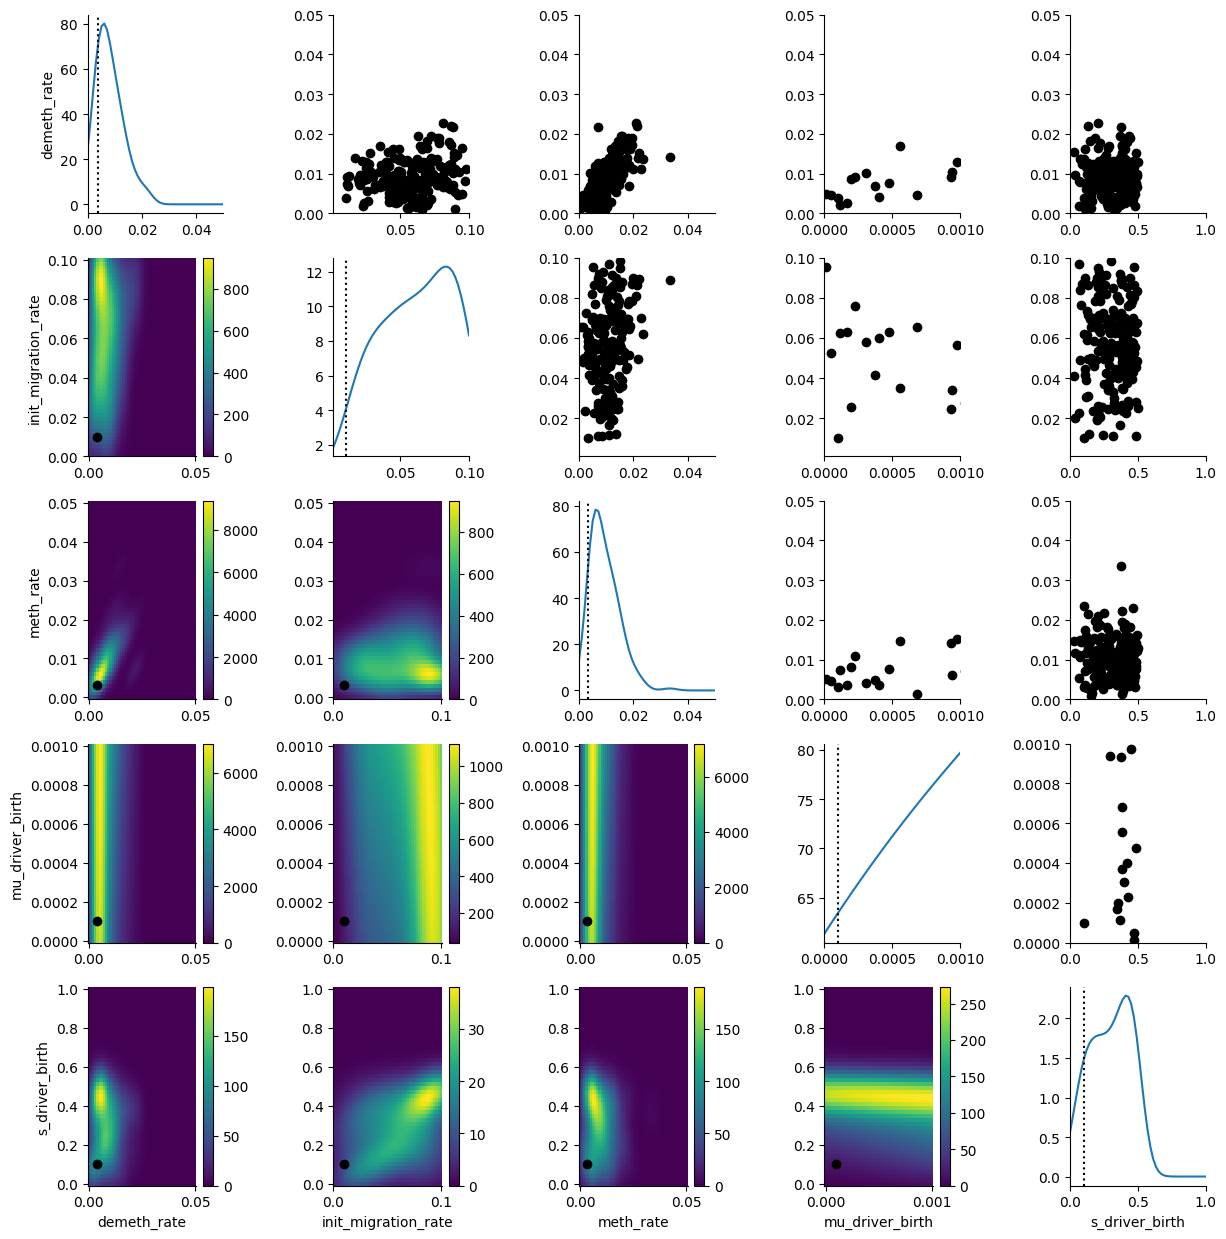
\includegraphics[width=\textwidth]{Chapter_4/figures/example_inference.png}
    \caption{Results of the example inference of the \texttt{methdemon} model.
    The ground truth parameter values are shown as dotted vertical lines in the
    plots on the diagonal.}
    \label{fig:example_inference}
\end{figure}
\clearpage
The results show a few interesting things. Firstly, the posterior distribution
of the epimutation rates has narrowed down to a small range, close to the ground
truth values. This is likely due to the way in which epimutation rates are
expressed in the fCpG array - too fast and the distribution becomes Gaussian,
too slow and few changes occur. The Wasserstein distance favours simulations
with a similar bias to the observed data, meaning that the ratio of the two is
likely to stay preserved. Additionally, the magnitude of the epimutation rates
is encoded in the inter-gland distance matrices in a similar way to the individual
deme fCpG distributions, with the difference between glands being more pronounced
close to the sweet-spot of the rates. \par
The posterior distributions of the other three parameters are less informative,
as they have remained broad. This could be the case for a few reasons. Firstly,
the data itself could be uninformative, meaning that the model is not capable of
capturing the relationship between the input parameters and the output data.
Despite prior testing showing that the outputs are sensitive to the input
parameters, this is a complex model and it is possible that the relationship
between the parameters and the output data is not straightforward. For example,
a slowly growing tumour (lower fission rate) with no to weak selection and a
moderate mutation rate could produce similar outputs to a fast-growing tumour
with strong selection and a high mutation rate. This is not a problem with the
model, but a feature of the tumour's growth dynamics. The priors in this test
were chosen to be broad, covering both realistic and unrealistic behaviour of
cancer. In reality, a lot of tumours grow under weak selection or effectively
neutral dynamics. Secondly, the distance between observed and simulated data
could be uninformative. The choice of summary statistics was a natural one, but
it is possible that weaker signatures in the data are not captured by the
distance metrics. This is a common problem in ABC, and is usually addressed by
refining the rejection step, in addition to a more informative prior. Finally,
having multiple possible parameter combinations which produce similar outputs
could lead to a broad posterior distribution. This is an issue commonly debated
in the literature, as selection is difficult to quantify in real tumour data.
None the less, the results of the example inference are useful in that they show
the ability of ABC to narrow down at least parts of the parameter space even in
the case of broad priors in a complex model.

\section{Discussion}
In this chapter, I have presented a new agent-based model, \texttt{methdemon},
which is capable of simulating the growth of a tumour and the corresponding
fluctuating methylation arrays. The model is developed with efficiency and
dynamic memory management in mind, and is based on well-established models of
tumour growth and evolution. The model is capable of simulating the growth of a
tumour in a reasonable time, and the outputs are sensitive to the input
parameters to varying degrees. I have also presented and tested an ABC workflow
for inferring the parameters of the model from observed data. The workflow is
capable of narrowing down the parameter space, and the results of an example
inference show important features which need to be addressed when using the
workflow on real data.
